\section{Approach Overview}
\label{overview:sec}

{\tool} has two main processes: training and predicting.

\subsection{Training Process}

Figure~\ref{overview-training} displays the general architecture of
{\tool}'s training process. The input of the training process is the
source code of the buggy method and one buggy statement. If a method
has multiple buggy statements, we treat one buggy statement and that
enclosing method at a time as a training instance. The output includes
the trained tree-based context learning model (\code{CCL} model to
learn the surrounding code context) and the trained tree-based code
transformation learning model (\code{CTL} model to learn the
bug-fixing code transformation) with their parameters. The training
process has two main steps:

\begin{figure}[t]
	\centering
	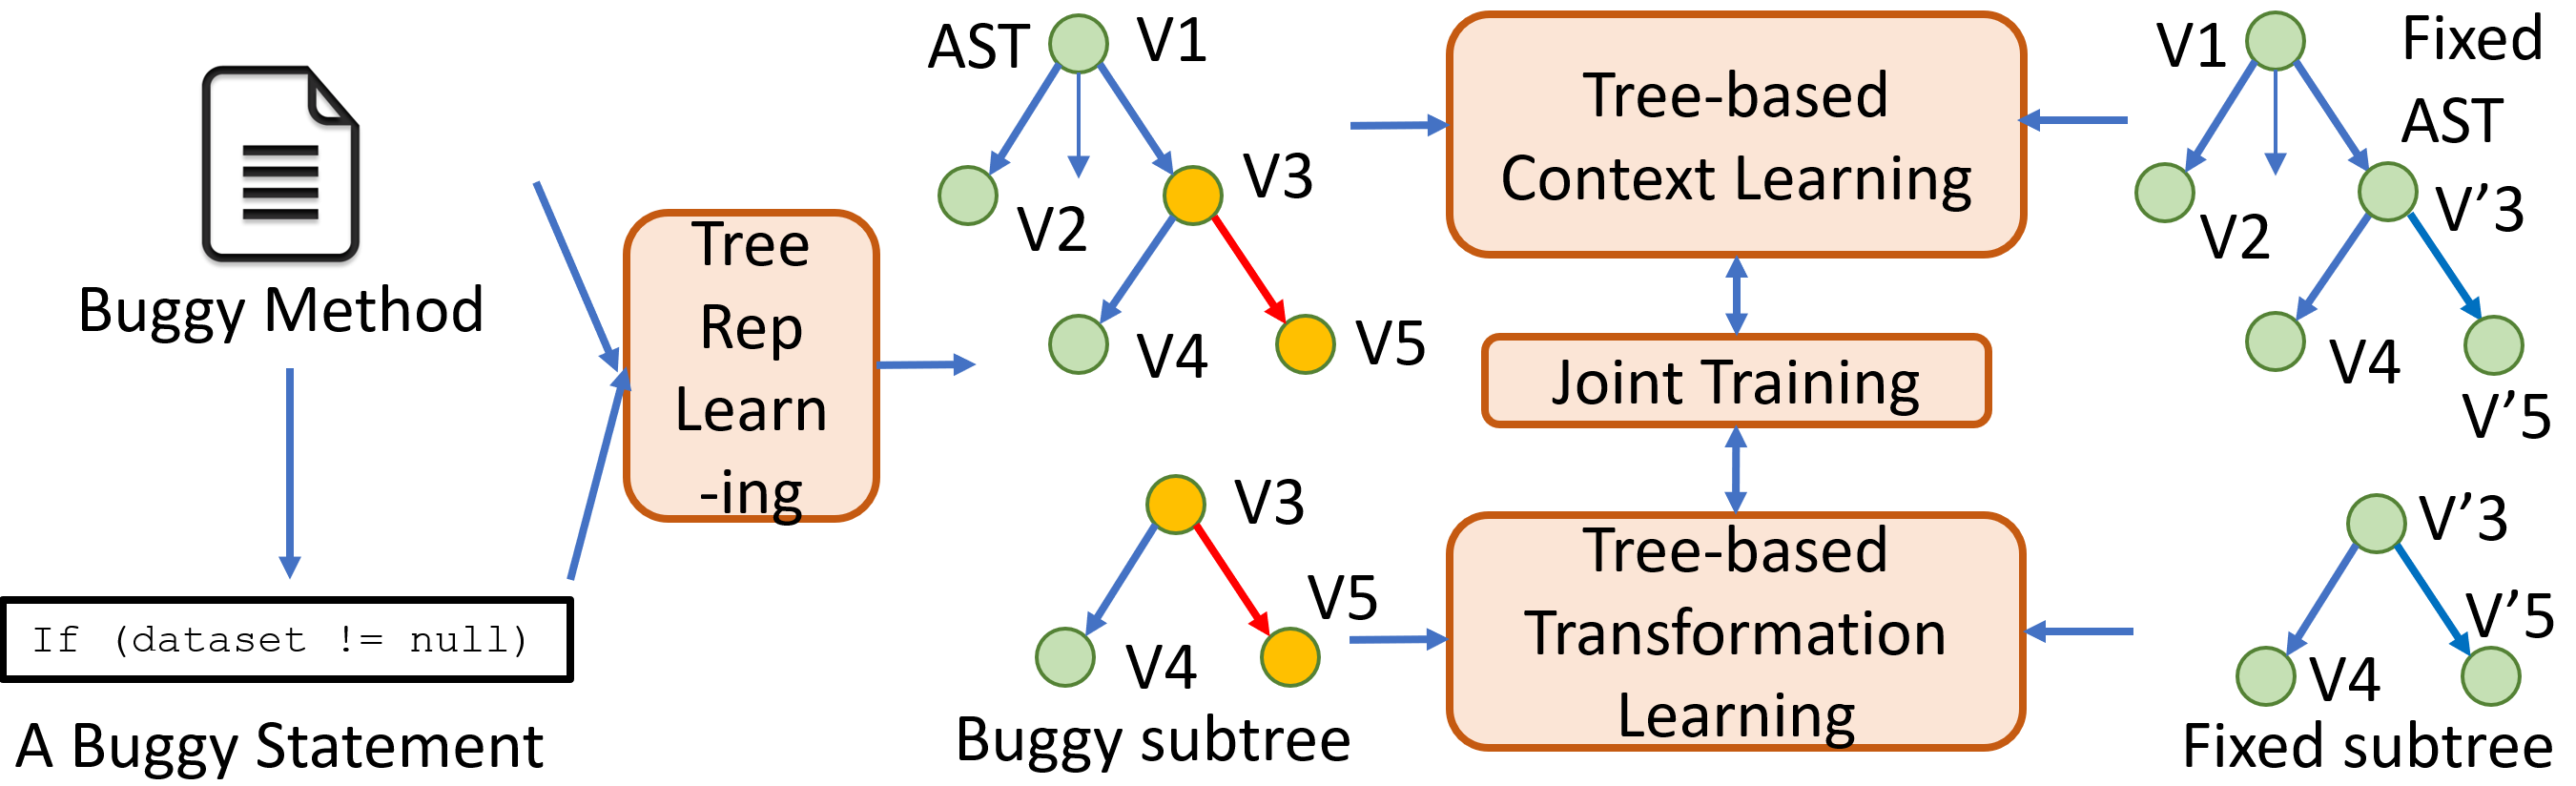
\includegraphics[width=3.4in]{graphs/overview-training.png}
	\caption{{\tool}: Training}
	\label{overview-training}
\end{figure}

\noindent {\bf Tree-based Representation Learning.} The goal of this
step is to take the source code under study and to build the
tree-based vector representations (embeddings) to be the input for our
dual models: \code{CCL} and \code{CTL}. To achieve that, we first
parse the given source code to obtain the abstract syntax tree (AST)
for the entire method and the subtree for the buggy statement.  We
then use a word embedding technique to produce the vector for each
node in the AST when we flatten the AST. The output of this step is
the AST for the method and the AST subtree for the buggy statement in
which each node is replaced by its embedding vector
(Figure~\ref{overview-training}).



\begin{figure}[t]
	\centering
	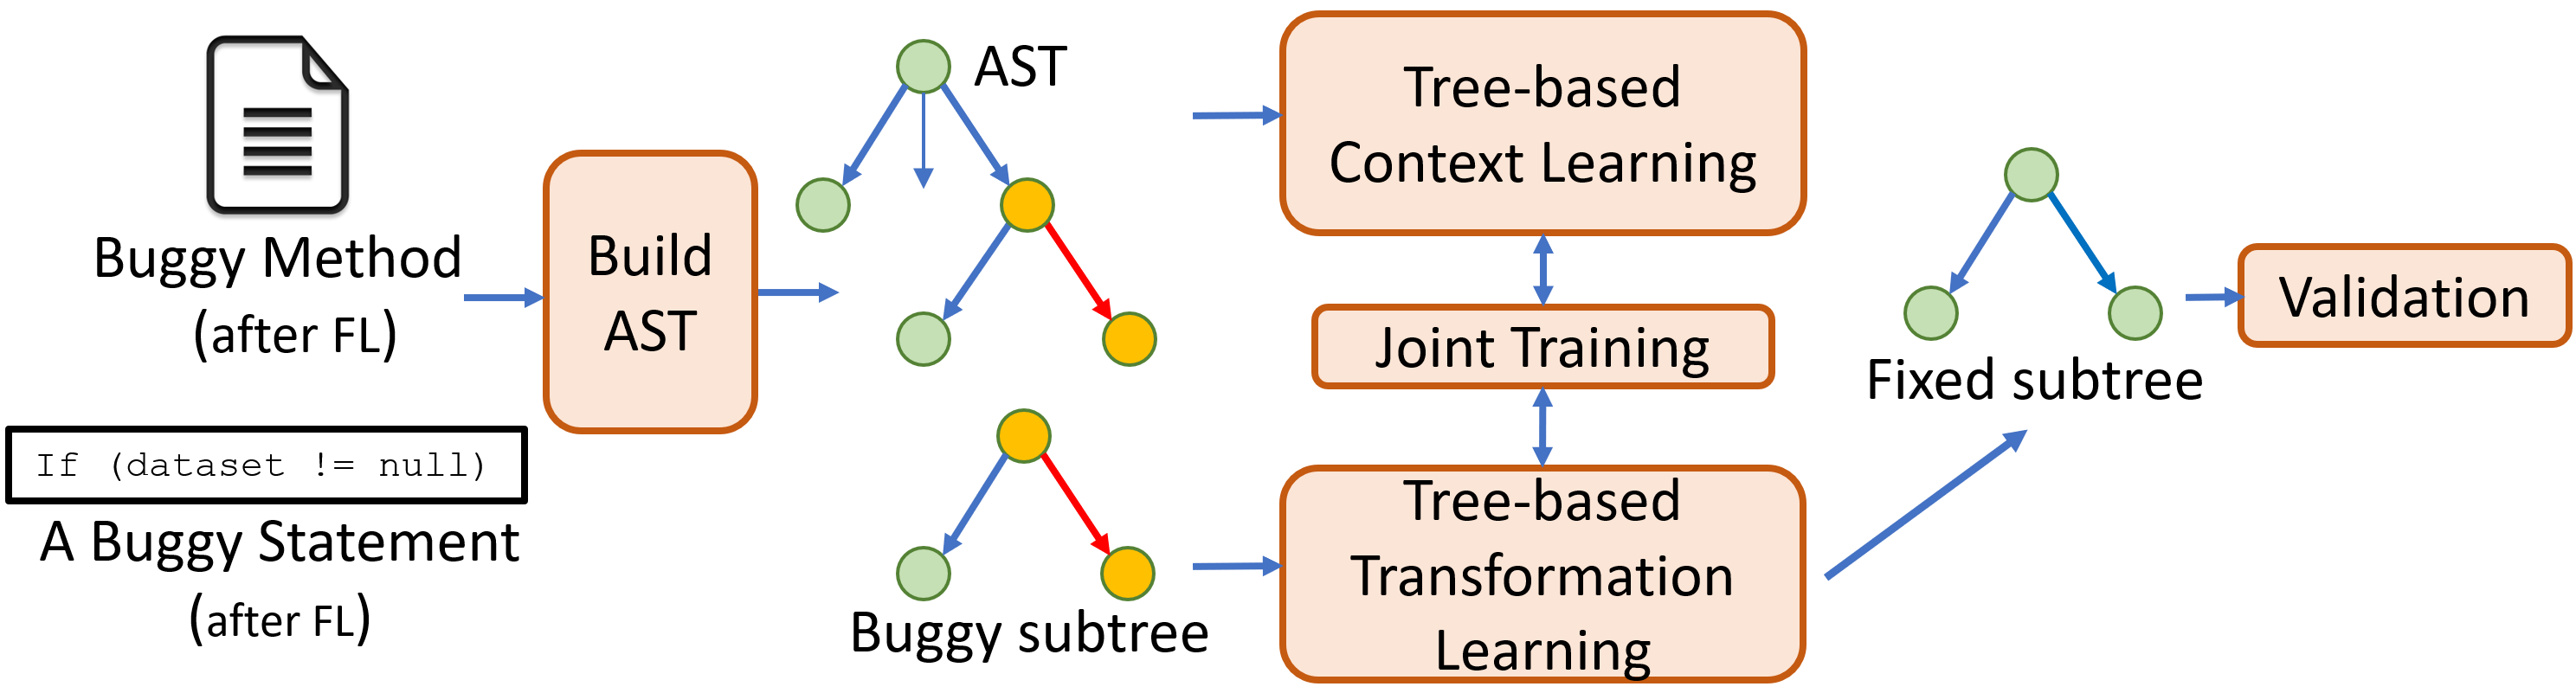
\includegraphics[width=3.4in]{graphs/overview-predict.png}
	\caption{{\tool}: Fixing}
	\label{overview-fixing}
\end{figure}

